\documentclass[a4paper, 11pt]{article}
\usepackage[left=2cm,text={17cm, 24cm},top=3cm,left= 2cm]{geometry}
\usepackage[IL2]{fontenc}
\usepackage[czech]{babel}
\usepackage[utf8]{inputenc}
\usepackage{graphicx}
\usepackage{subcaption}
\usepackage{float}
\usepackage{url}
\providecommand{\uv}[1]{\quotedblbase #1\textquotedblleft}
\DeclareUrlCommand\url{\def\UrlLeft{<}\def\UrlRight{>} \urlstyle{tt}}

\begin{document}
\thispagestyle{empty}
\begin{center}
\Huge
\textsc{Vysoké učení technické v Brně}\\
\huge
\textsc{Fakulta informačních technologií}\\
\LARGE
\vspace{\stretch{0.382}}
Modelování a simulace - 6. Počítačové služby\\ \Huge Porovnávání SQL a JAVA přístupů do databáze
\vspace{\stretch{0.618}}
\end{center}

{
\LARGE \hfill
Vojtěch Meluzín - xmeluz04\\
\today \hfill
Matěj Mlejnek - xmlejn04}

\newpage
\thispagestyle{empty}

\tableofcontents

\newpage
\setcounter{page}{1}
\section{Úvod}
V této práci je řešen projekt do předmětu \textbf{IMS - Modelování a simulace} \cite{ims_web} vyučovaném na Fakulta informačních technologií Vysokého učení technického v Brně \cite{fit_web}. Konkrétně se jedná o zadání \textbf{6. Počítačové služby} \cite{zadani_web}.

Tato práce se věnuje problematice vyhledávacích časů nad databází, kde jsme se zaměřili na zkoumání časových rozdílů mezi SQL dotazy a načítáním do RAM paměti s následným procházením po jednotlivých řádcích. Následné vygenerované data analyzujeme a modelujeme na jejich základě //TODO v simlibu\cite{simlib_web, simlib_zdroj}
\subsection{Zdroje faktů}
Jako model jsme si vybrali databázi Postgresql \cite{postgresql_web}. Pro přístup do této databáze jsme zvolili naprogramování aplikace v jazyce JAVA \cite{java_web} ve verzi JDK-1.8.0\_151 \cite{java_jdk_version}, ve které jsme si naprogramovali komunikaci se serverem. Programy pro sběr dat z této komunikace běželi na virtualním stroji Ubuntu 16.04.3 LTS \cite{ubuntu_web} a samotné posílání jednotlivých dotazů bylo zautomatizované pomocí scriptu psaném v GNU Bash version 4.3.48(1)-release (x86\_64-pc-linux-gnu) \cite{bash_web}.

\subsection{Ověření funkčnosti modelu}
//TODO zdrojová data jsou uz tak validni.

\section{Fakta}
//TODO naflakat spoustu grafu a popsat co vsecno znamana

?? odchylka
literatura atd 
osobni zprostredkovane pozorovani

\subsection{První běh}
\newpage
\begin{figure}[H]
\centering
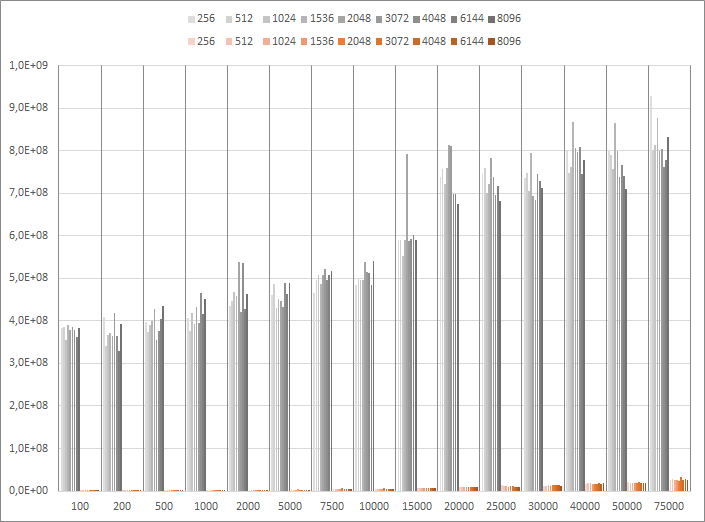
\includegraphics[width=100mm]{images/f1-100-75k.png}
\caption{LIKEE 1 - 100-75 000}
\end{figure}
\begin{figure}[H]
\centering
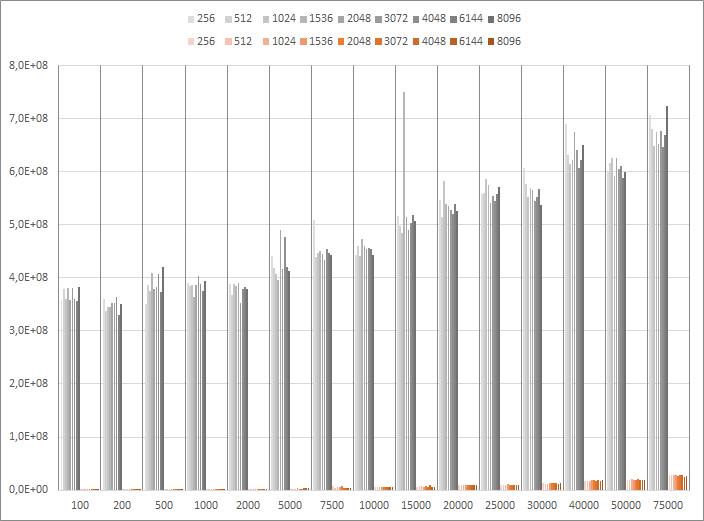
\includegraphics[width=100mm]{images/f10-100-75k.png}
\caption{LIKEE 10 - 100-75 000}
\end{figure}
\begin{figure}[H]
\centering
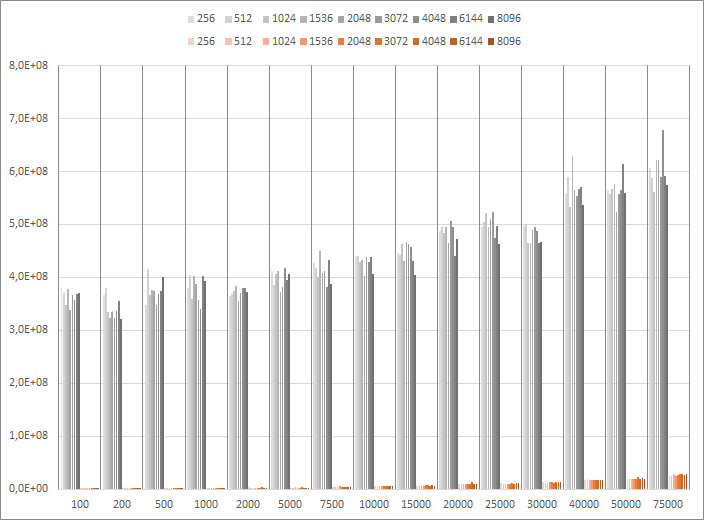
\includegraphics[width=100mm]{images/f100-100-75k.png}
\caption{LIKEE 100 - 100-75 000}
\end{figure}
\begin{figure}[H]
\centering
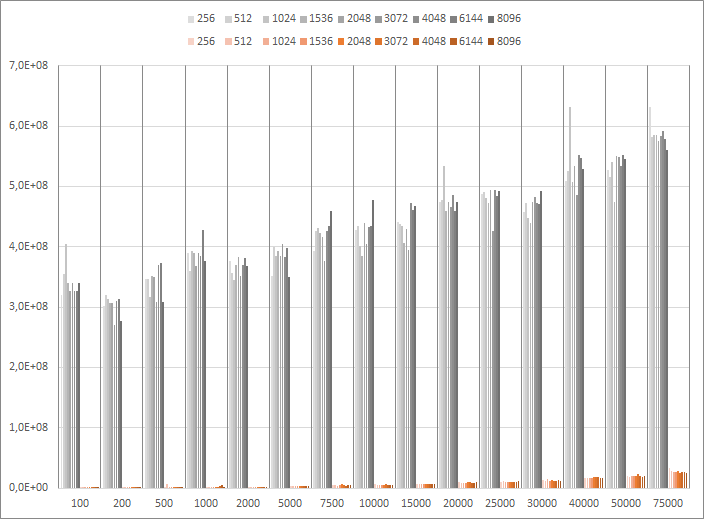
\includegraphics[width=100mm]{images/f1000-100-75k.png}
\caption{LIKEE 1000 - 100-75 000}
\end{figure}

\begin{figure}[H]
\centering
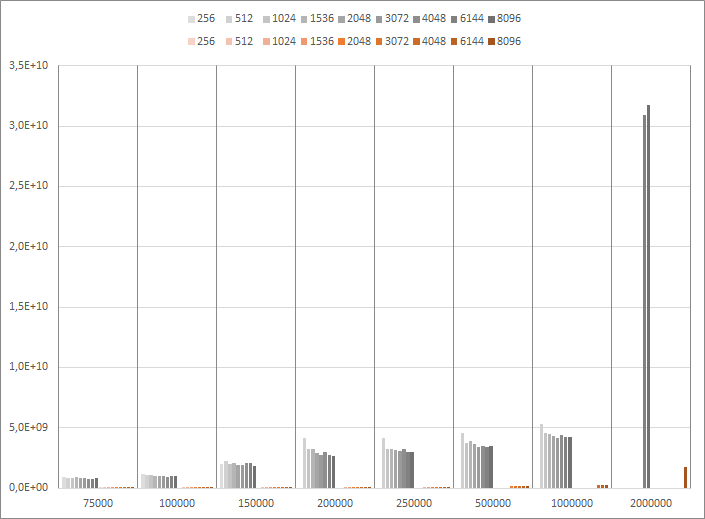
\includegraphics[width=100mm]{images/f1-75k-2kk.png}
\caption{LIKEE 1 - 75 000-2 000 000}
\end{figure}
\begin{figure}[H]
\centering
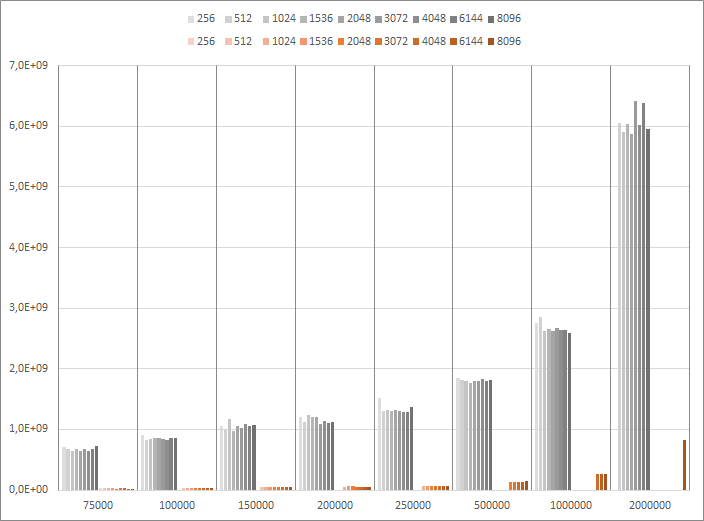
\includegraphics[width=100mm]{images/f10-75k-2kk.png}
\caption{LIKEE 10 - 75 000-2 000 000}
\end{figure}
\begin{figure}[H]
\centering
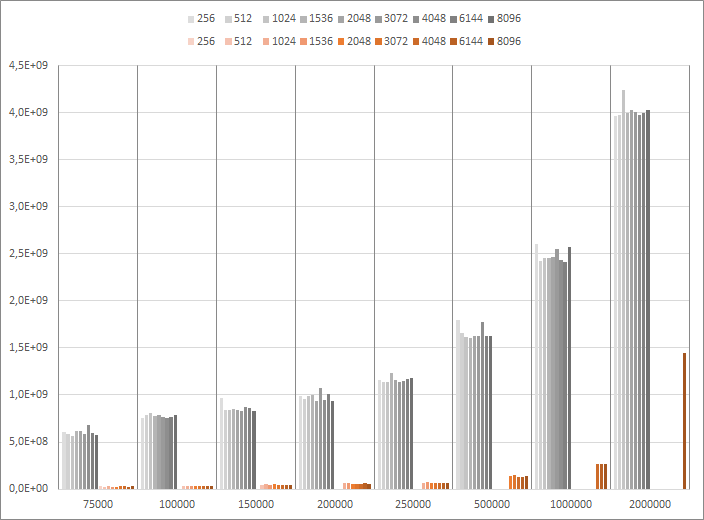
\includegraphics[width=100mm]{images/f100-75k-2kk.png}
\caption{LIKEE 100 - 75 000-2 000 000}
\end{figure} 
\begin{figure}[H]
\centering
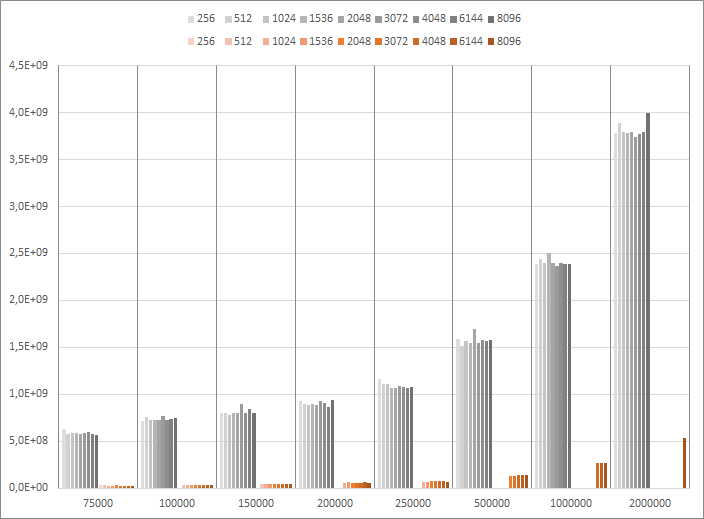
\includegraphics[width=100mm]{images/f1000-75k-2kk.png}
\caption{LIKEE 1000 - 75 000-2 000 000}
\end{figure}

\subsection{Vícenásobný běh}



\section{Koncepce modelu}
petriho sit



\section{Rodina}
Značí styl pro skupinu od sebe odvozených písem. Mezi základní patří: \\ 
\verb|\textrm| \hspace{0.5cm} \textrm{Roman family} - latinka;\\
\verb|\textsf| \hspace{0.5cm} \textsf{Sans serif family} - bezpatkové písmo;\\
\verb|\textttt| \hspace{0.3cm} \texttt{Typewriter family} - strojopisné písmo;
\cite{latex_kompletni_pruvodce, typograficky_manual}

\subsection{Varianty}
Tvary písem lze dále ovlivnit použitím jejich variant. Mezi základní patří: \\
\verb|\itshape| \hspace{0.5cm} \itshape{kurzíva;} \\
\verb|\slsshape| \hspace{0.28cm} \slshape{naklonění;} \\
\verb|\scshape| \hspace{0.5cm} \scshape přepnutí na velká písmena a kapitálky; \normalfont
\cite{latex_kompletni_pruvodce, typograficky_manual}

\subsection{Váha}
Váha písma určuje šířku neboli tloušťku písma. Lze použít např: \\
\verb|\mdseries| \hspace{0.5cm} přepnutí na střední(defaultní) tloušťku; \\
\verb|\bfseries| \hspace{0.5cm} přepnutí do \bfseries tučného \normalfont písma;
\cite{latex_kompletni_pruvodce, typograficky_manual}

\section{\TeX}
\TeX \- je typografický systém původně určený zejména pro kvalitní sazbu  nejen odborných publikací.
\cite{dipl_martin_cerny}

\section{Bib\TeX}
Bib\TeX \- je nástroj pro \LaTeX \- pomocí něhož se dájí vytvářet odkazy na použitou literaturu.    \\
Seznam citací se vytváří pomocí příkazu \verb|\bibliography{jméno souboru}|. Tentoe pomocí příkazu \verb|\cite{název navěští}|.


\pagebreak
\newpage
\bibliographystyle{czechiso}
\def\refname{Literatura}
\bibliography{proj4}

\end{document}